% case 1 results

\section{Case overview}

Case One examines knowledge sharing behaviour between eighteen people from seven organisations involved in a collaboration addressing cold-chain innovation. Fresh Produce is a family-owned business that supplies a range of green leafy vegetable products to caterers, restaurants, green grocers and supermarket chains. Products are supplied in cartons or in pre-packaged bags sold by the carton. Pre-packaged bags are supplied either as their own branded product or as a supermarket private-label product. Fresh Produce is based in a region that enjoys a temperate climate, enabling them to grow a greater variety of green leafy vegetables all year round. Fresh Produce competes with a handful of other firms for supply contracts with national supermarket chains. It views itself as a progressive business that combines innovation, expertise, and a good work ethic to provide the highest quality fresh produce to its customers.\medskip

Because green leafy vegetable products have a shelf-life of eight days post-production, Fresh Produce have to deliver products by refrigerated trucks to customers within two to three days of harvesting. Cartons are packed on wooden pallets stacked in two rows down the length of the refrigerated compartment. Maintaining uniform air temperatures between 1\si{\degree}C and 4\si{\degree}C in tightly-packed trucks is challenging. Refrigerated air tends to flows around the outside of a load and not through the load resulting in an uneven temperature distribution, which can lead to spoilage. Fresh Produce have initiated a program to improve on-farm product handling and packaging practices in an effort to reduce spoilage and improve the shelf-life of their products. The cold chain initiative is being driven by the general manager responsible for product processing and delivery at Fresh Produce. His goal is to ensure Fresh Produce is at the forefront of current best practice. Fresh Produce has excellent working relations with its freight forwarders, all of whom are keen to help the company improve on-farm product handling and packaging practices. The freight forwarders have a wealth of experience in cold chain logistics and are motivated to help Fresh Produce in order to maintain goodwill and avoid being penalised when products get rejected because of temperature issues. It is not always clear if rejections are a result of poor on-farm practices or because air temperatures were not properly maintained during transit. Working together and sharing practical knowledge is in everybody's best interest.\medskip

Fresh Produce uses advanced wireless micro-sensor technology provided by Calypso Systems to gain insight into air temperature variation inside loaded trucks. Calypso Systems is a foreign-based firm that specialises in monitoring the condition of perishable goods through the supply chain. They develop, manufacture, and sell miniaturised wireless sensor devices that can be placed inside individual food packages. Each device records time and temperature on a continuous basis for up to 30 days. Data can be retrieved from each device using wireless data readers up to 100m away and uploaded to a central database, where it can be queried in a variety of ways. Calypso Systems is helping Fresh Produce develop an independent monitoring system to identify problem shipments before they are unloaded. Fresh Produce have also enlisted the local university to model temperature distributions inside refrigerated trucks using the data provided by the wireless sensor devices. The university recently established a research group to investigate how sensor technology and data analytics can be combined to solve practical problems in perishable goods supply chains. Fresh Produce hope the modelling done by the research group will lead to better load configurations and packaging material to improve product performance.\medskip

The cold chain initiative involves both process and product performance innovation (Figure \ref{fig:innovationtypes}). Because the aim is to improve on-farm product handling and packaging practices, this case may be considered an example of incremental innovation. Though the cold chain initiative is ongoing, this case study focuses on knowledge sharing and creative interaction around the temperature modelling activity. Fresh Produce see this initiative as their first serious foray into open innovation and are keen to improve their knowledge sharing practices.\medskip

\section{Quantitative analysis}

\subsection{Descriptive statistics}

\subsubsection{Demographics}

Eighteen people were invited to participate in this case study, all of whom accepted the invitation. Only two of the participants were female. The age range of participants was from 27 to 62 years (median age was 47 years). Relevant work experience ranged from 1 to 25 years (median work experience was 9 years). Current job tenure ranged from 1 to 20 years (median tenure was 7.5 years). Figure \ref{fig:ageexperience} shows the distribution of age, work experience and job tenure of participants for each case study. \medskip

Figure \ref{fig:sphdistancecase1} depicts the euclidean (spherical) distance between every participant in the collaboration calculated using their work-place postcodes as a geographic reference. Most participants are either co-located or within reasonable driving distance of each other. Some participants (nodes 2, 12, 13 and 14) are located several hundreds of kilometres away in other parts of the country. One participant is based on another continent (node 10).\medskip

\begin{figure}
	\centering
	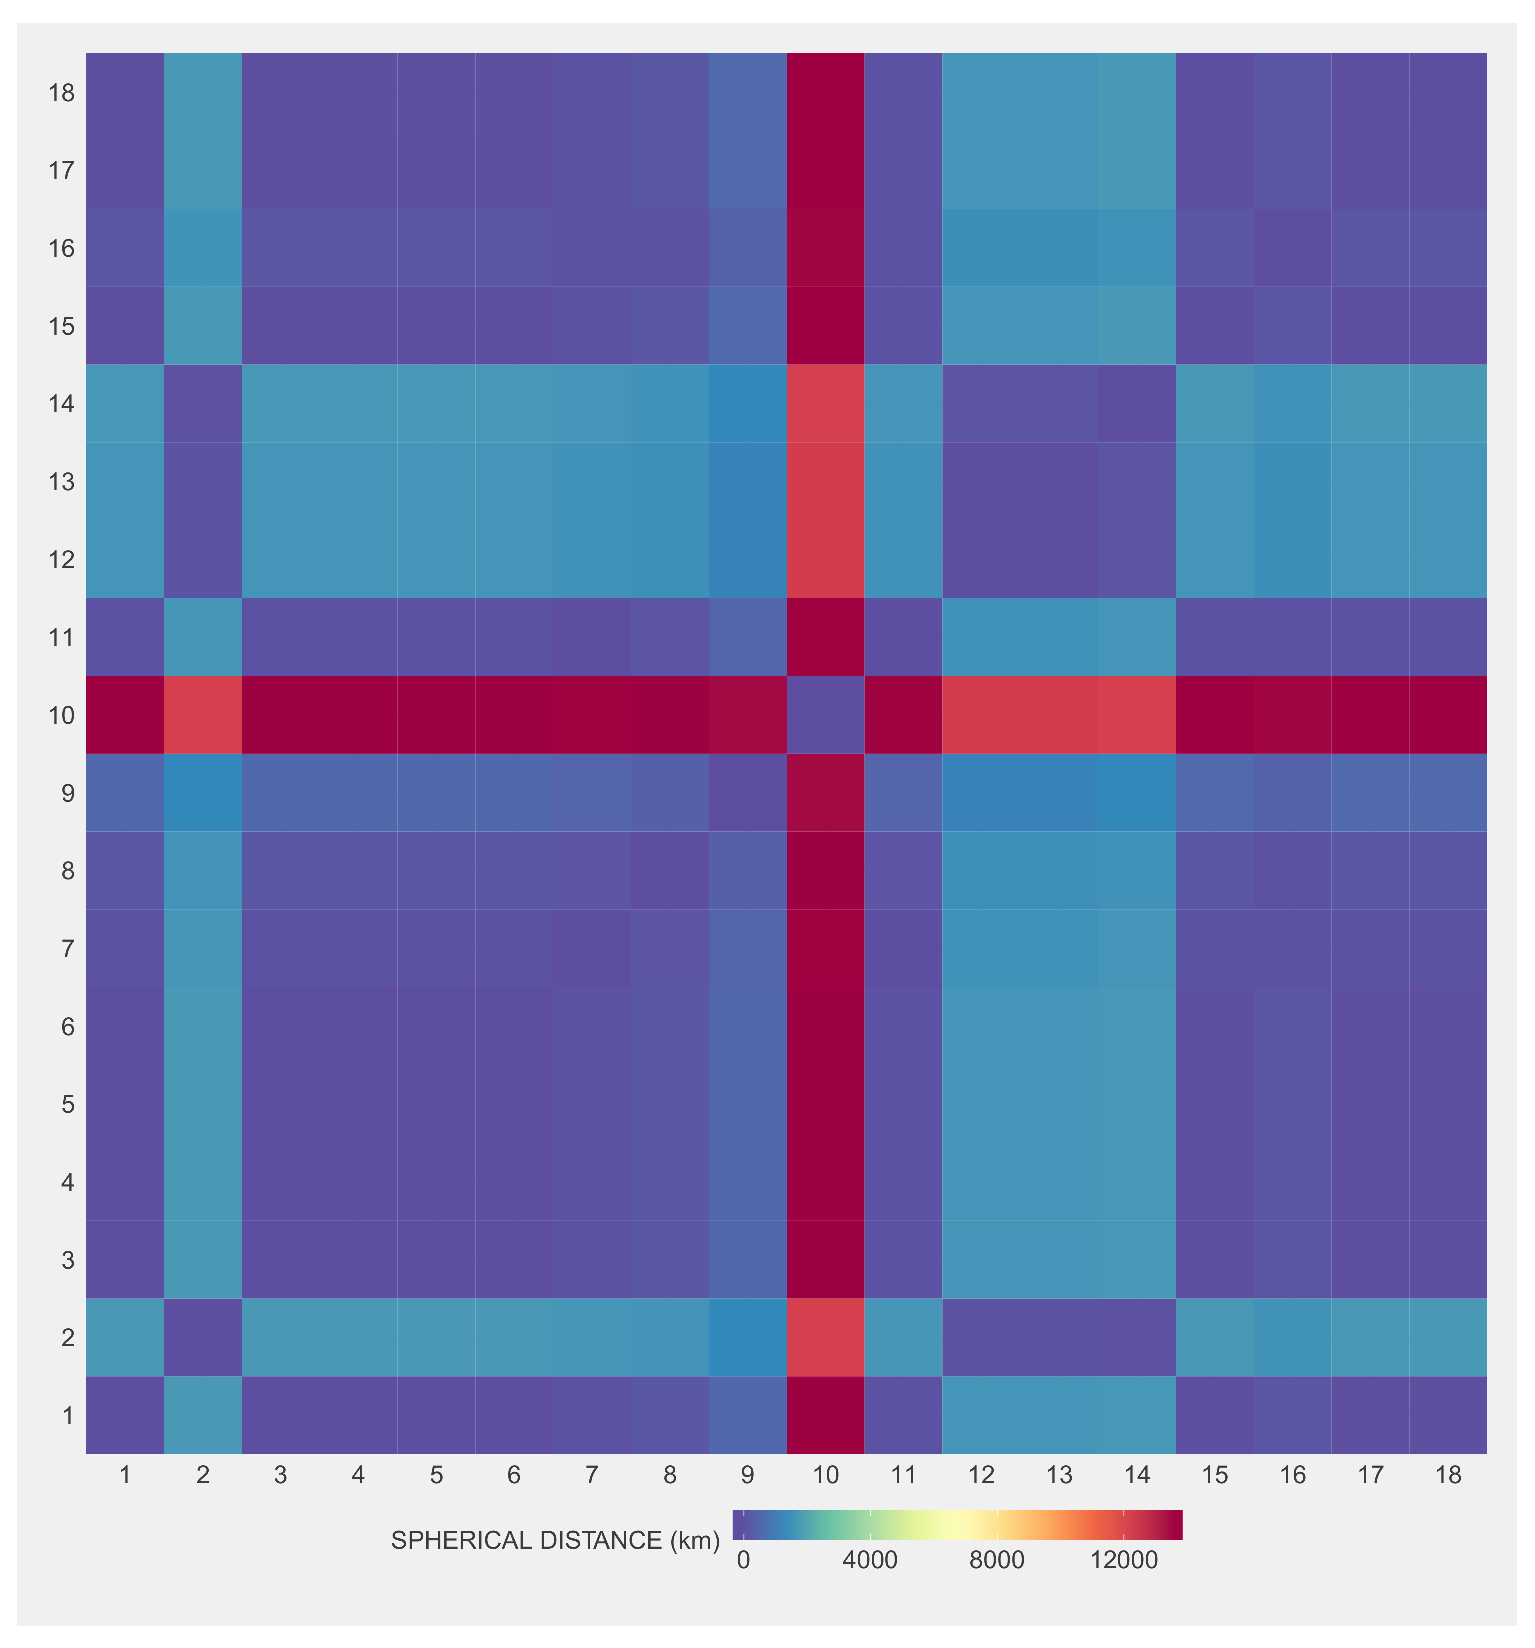
\includegraphics[width=0.7\linewidth]{Images/sph_distance_case1}
	\caption{Distance between nodes - Case One}
	\label{fig:sphdistancecase1}
\end{figure}

Participants in this case study have education levels ranging from high-school or secondary level to doctoral level (Figure \ref{fig:edlevelrose}). Many participants have some form of tertiary qualification. Participants come from diverse educational backgrounds including management and commerce, engineering and related studies, mixed field programmes, agriculture and environmental studies, natural and physical sciences, and education (Figure \ref{fig:edfieldrose}). 

\begin{figure}
\centering
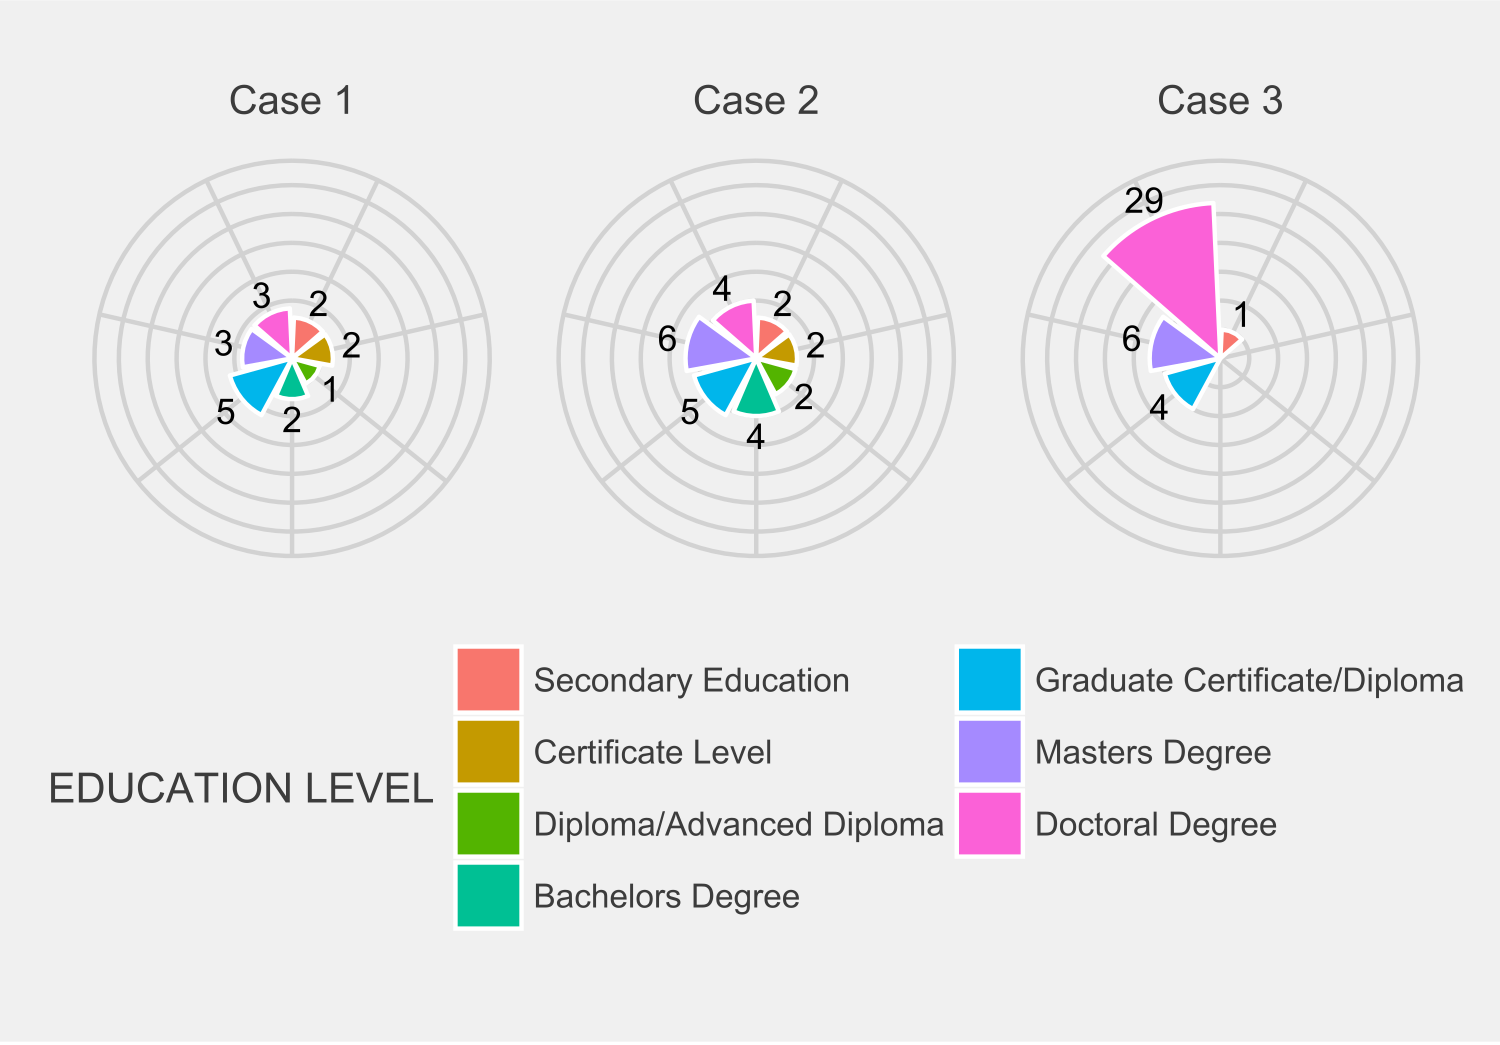
\includegraphics[width=0.7\linewidth]{Images/ed_level_rose}
\caption{Breakdown of educational level in each case}
\label{fig:edlevelrose}
\end{figure}

\begin{figure}
\centering
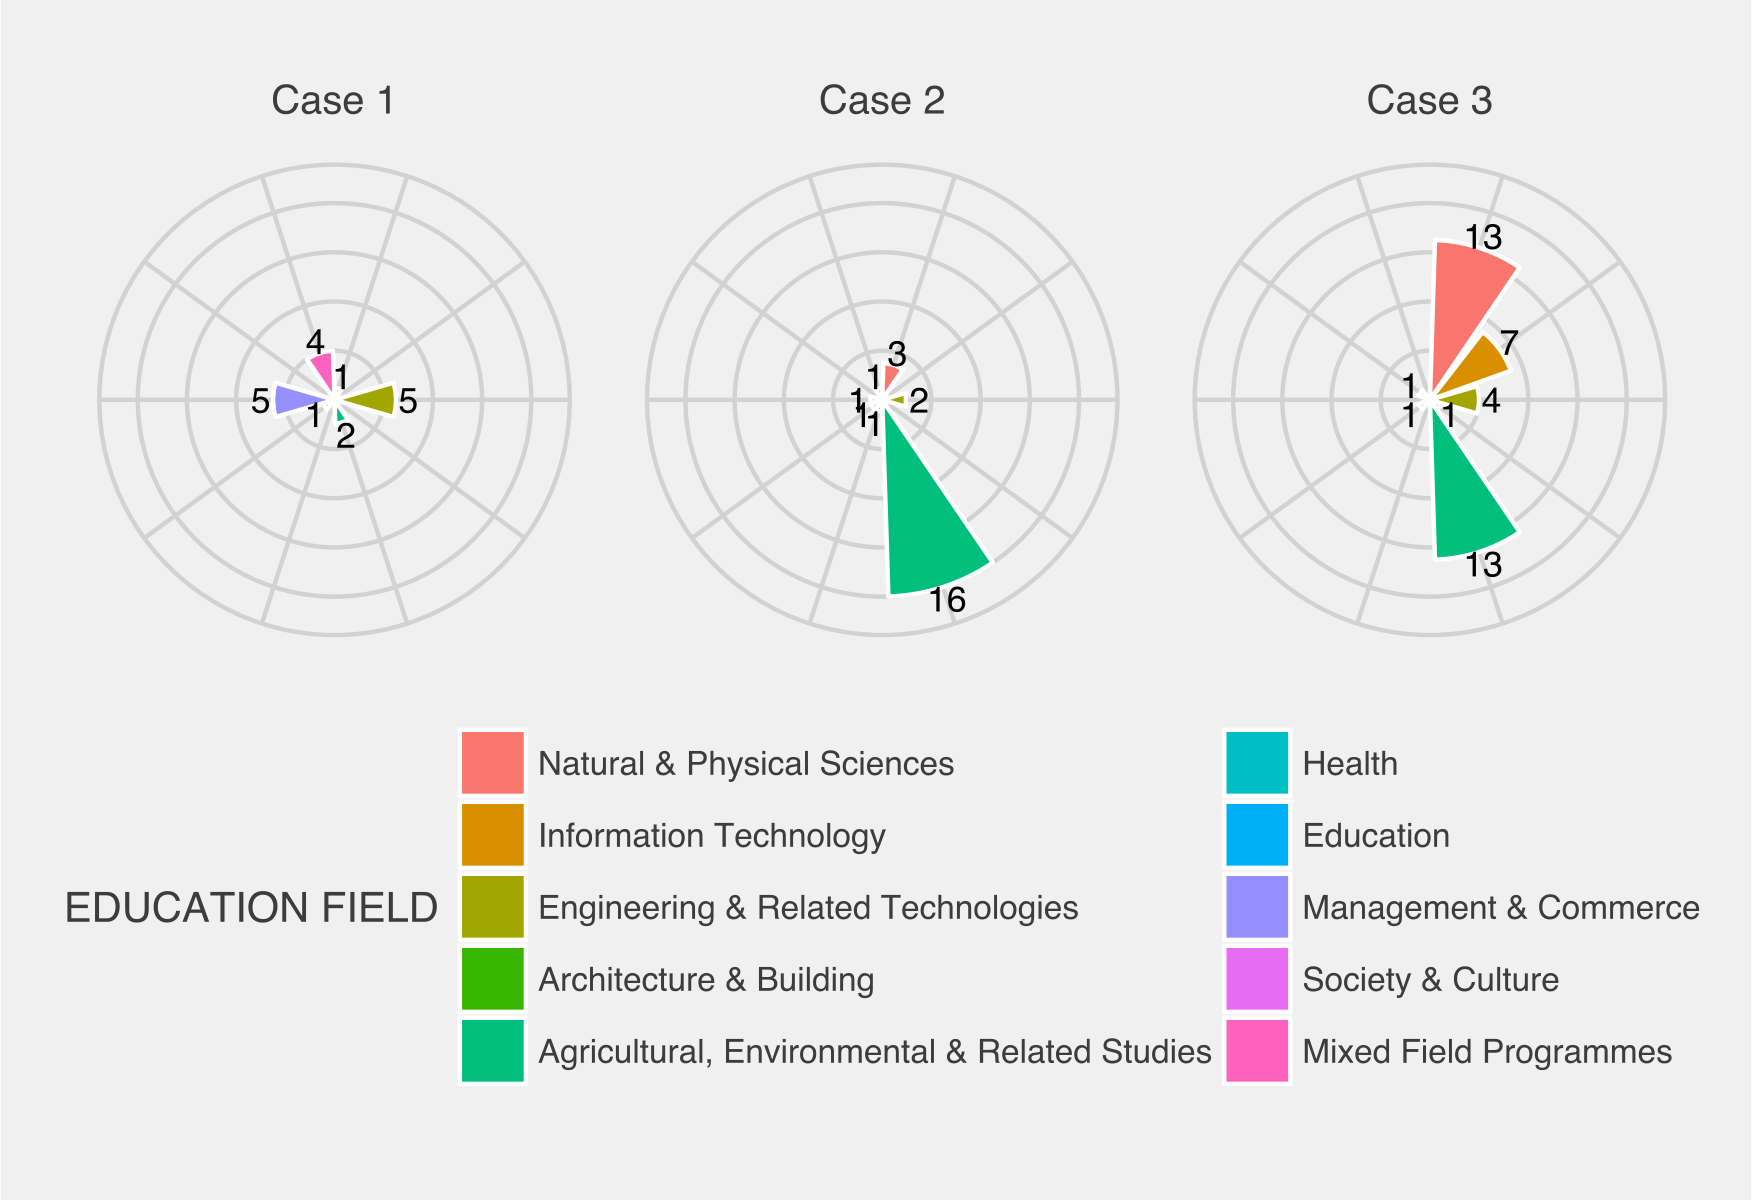
\includegraphics[width=0.7\linewidth]{Images/ed_field_rose}
\caption{Breakdown of broad education field in each case}
\label{fig:edfieldrose}
\end{figure}

\subsubsection{Basic network statistics}

Figure \ref{fig:thesisnetworkscase1} depicts the explicit knowledge provider, tacit  provider and idea contributor networks for Case One. Arrows indicate the direction of knowledge and idea flows. Nodes are sized according to Burt's constraint measure - the larger the node diameter, the greater the node's access to knowledge or ideas. Node colours indicate employer affiliation. Descriptive statistics for the three networks are presented in Table \ref{ds_c1}. The explicit knowledge provider network is the densest of the three networks (density = 0.20). Judging by the sparseness of the tacit knowledge provider network (density = 0.08), one can safely assume tacit knowledge does not feature very strongly in this collaboration. The idea contributor network has the most reciprocated ties of all three networks, which points to creative interaction being a key feature of this collaboration. All three networks are dominated by the same individual who has the greatest access to knowledge and ideas within the collaboration.\medskip

\begin{landscape}
	\begin{figure}
		\centering
		\includegraphics[width=1.0\linewidth]{Images/thesis_networks_case1}
		\caption{Network diagrams - Case 1}
		\label{fig:thesisnetworkscase1}
	\end{figure}
\end{landscape}

\begin{table}[]
	\small
	\centering
	\caption{Descriptive network statistics - Case One}
	\label{ds_c1}
	\begin{tabular}{@{}lcccccc@{}}
		\toprule
		& \multicolumn{1}{l}{} & \multicolumn{1}{l}{} & \multicolumn{1}{l}{} & \multicolumn{3}{c}{Dyad Census}	\\ \cline{5-7}
		Network						& Nodes			& Arcs			& Density	& Mutual		& Asymmetric	& Null		\\ \midrule
		Explicit Knowledge Provider & 18			& 61			& 0.20		& 12			& 37			& 104		\\
		Tacit Knowledge Provider    & 18			& 24			& 0.08		& 2				& 20			& 131		\\
		Idea Contributor            & 18			& 53			& 0.17		& 15			& 23			& 115		\\ \bottomrule
	\end{tabular}
\end{table}


\subsubsection{Two-path brokerage statistics}

Figure \ref{fig:gfbrokeragecase1} shows a breakdown of different brokerage roles in the explicit and tacit knowledge provider networks and idea contributor network according to employer affiliation. Table \ref{gf_params} explains what these roles signify. The explicit knowledge provider network shows a strong tendency for the liaison form of brokerage. This indicates people are happy to pass on explicit knowledge to other partner organisations. There is also a fair amount of representative brokerage, suggesting individuals are passing internally sourced explicit knowledge on to collaboration partners. Many individuals are operating as gatekeepers of explicit knowledge, implying much of the explicit knowledge being provided is being absorbed by receiving organisations. As Figure \ref{fig:thesisnetworkscase1} indicates, brokerage of tacit knowledge is quite limited. The main form of tacit knowledge brokerage is gatekeeping. Figure \ref{fig:gfbrokeragecase1} suggests there is much creative interaction with internally sourced ideas being passed between, and taken up by, partner organisations.


 

\begin{figure}
	\centering
	\includegraphics[width=0.7\linewidth]{Images/gf_brokerage_case1}
	\caption{Gould-Fernandez brokerage roles according to employer affiliation - Case One}
	\label{fig:gfbrokeragecase1}
\end{figure}


\subsection{Exponential random graph modelling}

\subsubsection{Autonomous motivation as a predictor of knowledge sharing}

Both the explicit and tacit knowledge provider networks were modelled to determine if autonomous motivation predicts knowledge sharing behaviour. Table \ref{c1_q1} contains the parameter estimates with standard errors in brackets for the explicit knowledge provider and tacit knowledge provider networks (Models A and B). The estimation procedure successfully converged for all the modelled parameters (refer to Table \ref{erm_params} for an explanation of all the model parameters used in this study). Goodness of fit statistics were less than 1 in absolute value for almost all the features not explicitly modelled, indicating the models fit the data reasonably well. Results are broken down according to purely structural effects, actor-relation effects, and network covariate effects. A significant effect is denoted by an asterisk when the parameter estimate is greater than two times the standard error in absolute value. Note the arc (edge) parameter is typically ignored because it is analogous to the intercept in a linear regression.\medskip

Looking at purely structural effects, there is a significant and positive effect for popularity spread in the explicit knowledge provider network. This implies there are some actors receiving significantly more explicit knowledge than others. Path closure is a significant and positive effect in the tacit knowledge provider network. This indicates a tendency to close structural holes when sharing tacit knowledge. Multiple connectivity, while positive, is not a significant effect in the tacit knowledge provider network. What all this implies is that people are generally happy to pass on explicit knowledge but are more economical when it comes to sharing tacit knowledge.\medskip

In terms of actor-relation effects, there is a significant and negative sender effect for education level in the explicit knowledge provider network, indicating more educated individuals are less likely to share explicit knowledge. Given the question used to generate the knowledge provider network asked respondents to name people who provide them with useful knowledge that helps them accomplish their tasks in the collaboration, it may be that individuals with higher levels of education are less likely to be approached for explicit knowledge. There is also strong and positive effect for employer-match and employer-mismatch reciprocity in the explicit knowledge network. This suggests people are more likely to share explicit knowledge with their work colleagues and when explicit knowledge is shared with people from other firms, this behaviour is likely to be reciprocated. There is a significant and positive receiver effect for both openness to experience and autonomous motivation in the tacit knowledge provider network. This is not surprising given the question used to generate the knowledge provider network. We are observing knowledge-seeking behaviour rather than knowledge-sharing behaviour. Essentially the modelling shows autonomously motivated individuals who are open to experience are more likely to seek out and acquire tacit knowledge. The tacit knowledge provider network also shows a strong and positive effect for identification with the collaboration, suggesting individuals who identify more strongly with the collaboration are more inclined to share tacit knowledge.\medskip

With respect to network covariate effects, hierarchy has a strong and positive effect in the explicit knowledge provider network. Individuals are more likely to share explicit knowledge with those they report to in the collaboration. As expected, spatial proximity has a significant and negative effect in the tacit knowledge provider network. Tacit knowledge is typically exchanged through face-to-face interaction and this is more likely to happen between people in close proximity.\medskip

In conclusion, the exponential random graph modelling indicates autonomous motivation has no effect with respect to explicit knowledge but does appear to have a significant and positive effect on tacit knowledge seeking behaviour.

\begin{table}[]
	\centering
	\caption{Autonomous motivation as a predictor for knowledge sharing - Case 1}
	\label{c1_q1}
	\begin{threeparttable}
		\begin{tabular}{@{}lrlrl@{}}
			\toprule
			& \multicolumn{4}{c}{Estimate (SE)} \\ \cline{2-5} 
			& \multicolumn{2}{c}{\begin{tabular}[c]{@{}c@{}}Model A\end{tabular}} & \multicolumn{2}{c}{\begin{tabular}[c]{@{}c@{}}Model B\end{tabular}} \\\midrule
			\textbf{Purely structural effects (endogenous)} &           &             &          &           \\
			Arc (edge)                                      & -0.316    & (3.432)     & -23.100  & (5.607)*  \\
			Reciprocity (mutuality)                         & -1.572    & (1.109)     & -0.871   & (1.655)   \\
			TwoPath (simple connectivity)                   & -0.157    & (0.243)     & -2.909   & (1.709)   \\
			AinS (popularity spread)                        & 1.431     & (0.636)*    & -1.029   & (0.728)   \\
			AoutS (activity spread)                         & -1.568    & (1.234)     & -0.184   & (0.602)   \\
			AT-T (path closure)                             & 0.709     & (0.383)     & 2.274    & (0.771)*  \\
			AT-C (cyclic closure)                           & -0.471    & (0.250)      & -2.281   & (4.460)    \\
			A2P-T (multiple connectivity)                   & 0.440     & (0.247)     & 3.177    & (1.742)   \\
															&           &             &          &           \\
			\textbf{Actor-relation effects (exogenous)}     &           &             &          &           \\
			age (difference)                                & 0.001     & (0.021)     & 0.031    & (0.043)   \\
			work.experience (sender)                        & -0.033    & (0.05)      & 0.014    & (0.049)   \\
			work.experience (receiver)                      & 0.002     & (0.022)     & -0.031   & (0.074)   \\
			education.level (sender)                        & -0.364    & (0.149)*    & 0.147    & (0.166)   \\
			education.level (receiver)                      & 0.062     & (0.088)     & 0.462    & (0.228)*  \\
			personality.openness (sender)                   & 0.137     & (1.864)     & 2.437    & (2.192)   \\
			personality.openness (receiver)                 & -0.638    & (1.165)     & 9.232    & (3.470)*   \\
			self.efficacy (sender)                          & 0.440     & (2.281)     & -1.635   & (4.048)   \\
			self.efficacy (receiver)                        & -1.896    & (1.411)     & -7.533   & (4.884)   \\
			identification.collab (product)                 & -1.287    & (1.319)     & 5.726    & (2.735)*  \\
			autonomous.motivation (sender)                  & 1.005     & (1.571)     & 4.056    & (3.352)   \\
			autonomous.motivation (receiver)                & -0.889    & (1.06)      & 17.472   & (5.73)*   \\
			broad.education.field (match)                   & 0.560     & (0.449)     & 1.243    & (0.695)   \\
			employer (match)                                & 2.944     & (0.7)*      & 1.020    & (0.805)   \\
			employer (mismatch reciprocity)                 & 3.726     & (1.181)*    & -5.376   & (11.823)  \\
															&           &             &          &           \\
			\textbf{Network covariate effects (exogenous)}  &           &             &          &           \\
			report.to.net (heirarchy)                       & 1.274     & (0.503)*    & 1.145    & (0.863)   \\
			log.spherical.distance.net (spatial proximity)  & -0.008    & (0.078)     & -0.366   & (0.149)*  \\ \bottomrule
		\end{tabular}
		\begin{tablenotes}
			\small
			\item [*] Significant effect.
		\end{tablenotes}
	\end{threeparttable}
\end{table}


\subsubsection{Brokerage versus level of tacit knowledge exchange}

Work in progress.

\subsubsection{Role of tacit knowledge in creative interaction}

The idea contributor network was modelled to assess the influence of tacit knowledge on creative interaction (Model E). Table \ref{c1_q3} contains the parameter estimates with standard errors in brackets for Model E. The estimation procedure successfully converged for all the modelled parameters. Goodness of fit statistics were under 2 in absolute value for features not explicitly modelled, indicating Model E fits the data well. Results are again broken down according to purely structural effects, actor-relation effects, and network covariate effects.\medskip 

Looking at the purely structural effects, there is a significant and positive effect for path closure in Model E. This implies idea generation in this instance is largely a social process that involves joining a friend of a friend to a friend. With reference to actor-relation effects, there is a significant and positive sender effect in Model E for education level, suggesting individuals with a higher level of education are more likely to contribute ideas. In contrast, there is a strong and negative receiver effect for education level, indicating individuals with a higher level of education are less likely to receive ideas.\medskip

In terms of network effects, there is significant and positive dyadic covariate effect for both the explicit and tacit knowledge provider networks. In other words, idea contribution ties are more likely to emerge in the presence of existing knowledge sharing ties. However, the effect is stronger for the tacit knowledge provider network, implying there is a stronger tendency for creative interaction to happen between people who exchange tacit knowledge. Again one must not read too much into this, given the low density of the tacit knowledge provider network in this instance.\medskip     

\begin{table}[]
	\centering
	\caption{A model examining role of tacit knowledge in creative interaction - Case 1}
	\label{c1_q3}
	\begin{threeparttable}
		\begin{tabular}{@{}lrl@{}}
			\toprule
			& \multicolumn{2}{@{}c@{}}{Estimate (SE)} \\ \midrule
			\textbf{Purely structural effects (endogenous)}      &                &                  \\
			Arc (edge)                                           & -7.231         & (5.300)          \\
			Reciprocity (mutuality)                              & 2.403          & (1.475)          \\
			TwoPath (simple connectivity)                        & -0.608         & (0.462)          \\
			AinS (popularity spread)                             & -2.307         & (1.164)          \\
			AoutS (activity spread)                              & -0.783         & (0.747)          \\
			AT-T (path closure)                                  & 1.347          & (0.469)*         \\
			AT-C (cyclic closure)                                & -0.443         & (0.301)          \\
			A2P-T (multiple connectivity)                        & 0.570          & (0.467)          \\
			&                &                  \\
			\textbf{Actor-relation effects (exogenous)}          &                &                  \\
			age (difference)                                     & 0.030          & (0.040)          \\
			work.experience (sender)                             & -0.034         & (0.062)          \\
			work.experience (receiver)                           & 0.095          & (0.079)          \\
			education.level (sender)                             & 0.433          & (0.212)*         \\
			education.level (receiver)                           & -0.562         & (0.236)*         \\
			personality.openness (sender)                        & 3.640          & (2.502)          \\
			personality.openness (receiver)                      & 4.425          & (3.755)          \\
			self.efficacy (sender)                               & -2.751         & (3.084)          \\
			self.efficacy (receiver)                             & 3.890          & (4.098)          \\
			identification.collab (product)                      & -0.162         & (2.139)          \\
			autonomous.motivation (sender)                       & -1.589         & (2.343)          \\
			autonomous.motivation (receiver)                     & 0.560          & (2.971)          \\
			broad.education.field (match)                        & 1.147          & (0.630)          \\
			employer (match)                                     & -1.818         & (1.218)          \\
			employer (mismatch reciprocity)                      & -1.771         & (1.767)          \\
			&                &                  \\
			\textbf{Network covariate effects (exogenous)}       &                &                  \\
			tacit.knowledge.net (tacit knowledge provider)       & 9.062          & (1.883)*         \\
			explicit.knowledge.net (explicit knowledge provider) & 6.041          & (1.386)*         \\
			report.to.net (hierarchy)                            & 0.970          & (0.863)          \\
			log.spherical.distance.net (spatial proximity)       & 0.017          & (0.123)          \\ \bottomrule
		\end{tabular}
		\begin{tablenotes}
			\small
			\item [*] Significant effect.
			\
		\end{tablenotes}
	\end{threeparttable}
\end{table}


\section{Qualitative analysis}

\begin{landscape}
	\begin{table}[]
		\centering
		\caption{Case 1 interview participants.}
		\label{c1_interviews}
		\begin{threeparttable}
			\begin{tabular}{@{}cccccccccccc@{}}
				\toprule
				Node & Employer & \begin{tabular}[c]{@{}c@{}}Interview \\ Date\end{tabular} & Age & \begin{tabular}[c]{@{}c@{}}Relevant\\ Work \\ Experience\end{tabular} & \begin{tabular}[c]{@{}c@{}}Current \\ Job \\ Tenure\end{tabular} & \begin{tabular}[c]{@{}c@{}}Education\\ Level\end{tabular} & \begin{tabular}[c]{@{}c@{}}Broad\\ Education\\ Field\end{tabular} & \begin{tabular}[c]{@{}c@{}}In-degree\\ Centrality\end{tabular} & \begin{tabular}[c]{@{}c@{}}Out-degree\\ Centrality\end{tabular} & \begin{tabular}[c]{@{}c@{}}Eigenvector\\ Centrality\end{tabular} & \begin{tabular}[c]{@{}c@{}}Burt's\\ Constraint\\ Measure\end{tabular} \\ \midrule
				1    & 1        & 15/12/15  & 54  & 9     & 4                & 6         & 3                 & 17             & 14              & 1.00             & 0.20  \\
				3    & 1        & 26/04/16  & 51  & 10    & 19               & 2         & 5                 & 11             & 7               & 0.68             & 0.31  \\
				8    & 2        & 11/03/16  & 62  & 12    & 12               & 3         & 12                & 5              & 7               & 0.54             & 0.34  \\
				10   & 3        & 01/03/16  & 44  & 16    & 9                & 7         & 8                 & 1              & 1               & 0.16             & 1.00  \\
				15   & 7        & 24/02/16  & 51  & 25    & 1                & 7         & 3                 & 6              & 5               & 0.45             & 0.45  \\
				16   & 7        & 07/09/16  & 53  & 16    & 1                & 8         & 12                & 5              & 4               & 0.40             & 0.50  \\ \bottomrule
			\end{tabular}
			\begin{tablenotes}
				\small
				\item Notes:
				\item 1. Numbers in the education level/broad education field columns are the same as those used in the Australian Standard Classification for Education.
				\item 2. Statistics for the undifferentiated knowledge provider network.
				\item 3. In-degree centrality refers to the number of incoming knowledge ties. Out-degree centrality refers to the number of outgoing knowledge ties.
				\item 4. Eigenvector centrality refers to the relative importance of a node (connectivity with other high degree-centrality nodes) on a scale of 0 to 1.
				\item 5. Burt's constraint measure refers to access to network resources on a scale of 0 to 1. Lower values mean greater access to network resources.
			\end{tablenotes}
		\end{threeparttable}
	\end{table}
\end{landscape}
